\documentclass[12pt]{article}

\usepackage{xeCJK}%字體設定
\setCJKmainfont{cwTeXKai}
\setCJKmainfont{cwTeXKai}[AutoFakeBold=1.5]


\setmainfont{Times New Roman}  % 英文正文字體

\usepackage[top=2cm,bottom=2cm,left=2cm,right=2cm,a4paper]{geometry}%版面設定

\usepackage{indentfirst}%縮排

\usepackage{setspace}%行距設計
\onehalfspacing%半行距
\setlength{\parskip}{3pt}%段落之間

\usepackage{moresize}%字體大小

\usepackage{graphicx}

\usepackage{amssymb}%數學符號

\usepackage{amsmath} % 數學符號
\usepackage{booktabs}         % 漂亮的表格（\toprule, \midrule, \bottomrule）
\usepackage{siunitx}          % 國際單位制 (建議處理單位更漂亮)

\usepackage{multicol}%引入函數使下面那些可以變成雙欄

\usepackage{float}%圖片固定

% \renewcommand{\thesection}{\Roman{section}}


%%%%%%%%%%%%%%%%%%%%%%%%%%%%%%正文%%%%%%%%%%%%%%%%%%%%%%%%%%%%%%%%%%%
\begin{document}

\begin{titlepage}
\begin{center}

\vspace*{0.5cm}
\HUGE \textbf{普通物理實驗結報}\\
\vspace{1cm}
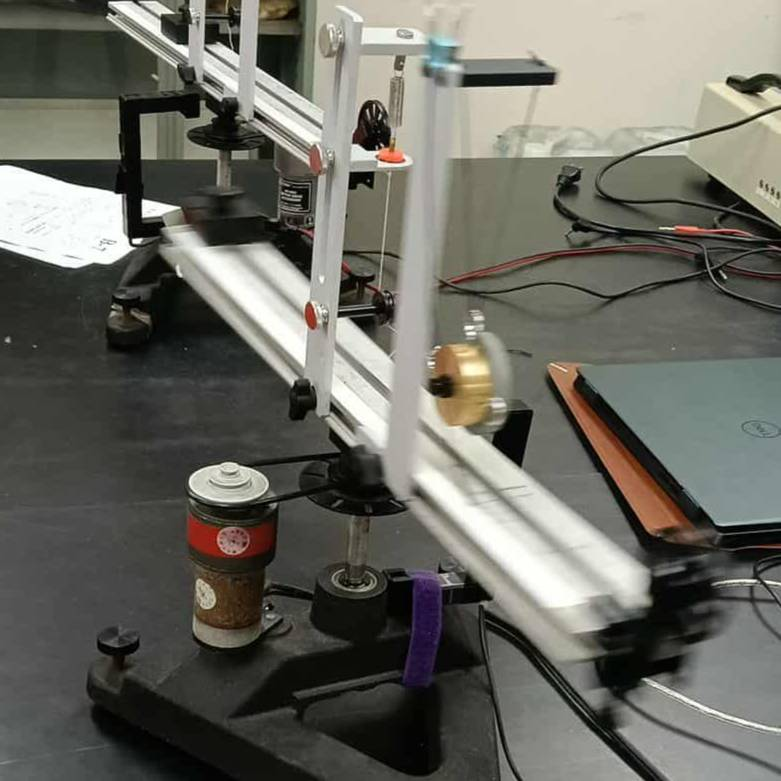
\includegraphics[width=9cm]{向心力圖表/轉轉轉.jpg}\\[0.5cm]
\HUGE \textbf{向心力}\\

\vfill
\huge 第三組\\[0.5cm]
\begin{table}[h]
\centering
\Large
\begin{tabular}{|c|c|}
\hline
組員:              & 貢獻度  \\
吳 & 33\% \\
卓 & 33\% \\
程 & 33\% \\ \hline
\end{tabular}
\end{table}

\end{center}

\end{titlepage}

%%%%%%%%%%%%%%%%%%%%%%%%%%%%%%%%%%%%%%%%%%%%%%%%%%%%%%%%%%%%%%%%

\large
\section{\textbf{實驗目的}}
研究物體作等速率圓周運動時，向心力、物體質量、旋轉半徑間的關係。

%%%%%%%%%%%%%%%%%%%%%%%%%%%%%%%%%%%%%%%%%%%%%%%%%%%%%%%%%%%%%%%%

\section{\textbf{實驗原理}}
根據牛頓第二運動定律，物體的加速度方向與合力方向相同，所以在等速率圓周運動中，物體恆受到指向圓心的法向加速度( Figure\ref{fig:centrifugal_force_1})。

在此實驗中，我們透過馬達來改變角速度、彈力提供向心力，並觀察旋轉過程中彈簧上的定位環與橘色指示片是否重合，兩者重合時表示物體所受到的向心力與靜止狀態下砝碼與砝碼吊盤的重量相等。
\begin{figure}[h]
    \centering
    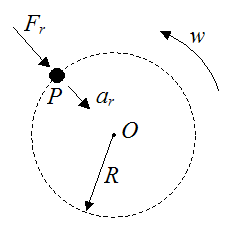
\includegraphics[width=0.2\linewidth]{向心力圖表/centrifugal_force_1.png}
    \caption{centrifugal force}
    \label{fig:centrifugal_force_1}
\end{figure}



%%%%%%%%%%%%%%%%%%%%%%%%%%%%%%%%%%%%%%%%%%%%%%%%%%%%%%%%%%%%%%
\section{\textbf{理論分析}}

\noindent
在本實驗中，法碼與吊盤所受的重力為
\[
F_g = mg
\]
而靜止時的彈力 $F_k$ 會與其平衡，因此可得$F_k = F_g$
\noindent
\\當系統開始旋轉並達到平衡時，旋轉法碼會受到向心力，
其來源為彈力 $F_k'$，因此:
\[
F_k' = Mr\omega^2
\]
又由平衡條件可得 $F_k' = F_k$。\\
綜合以上關係，可得到
\[
mg = Mr\omega^2 = Mr\frac{4\pi^2}{T^2}
\]
由此可推得旋轉質量、半徑與法碼質量之間的關係：
\[
M \propto \frac{mT^2}{r}, \quad
r \propto \frac{mT^2}{M}, \quad
m \propto \frac{Mr}{T^2}
\]

\bigskip
\noindent
其中各物理量定義如下：
\begin{multicols}{2}  % 2 欄，可改成 3 欄
\renewcommand{\labelitemi}{}  % 去掉圓點
\begin{itemize}
    \item $F_k$：靜止時的彈力(\si{\newton})
    \item $F_g$：法碼與平盤所受重力(\si{\newton})
    \item $F_k'$：旋轉時的彈力(\si{\newton})
    \item $M$：旋轉法碼質量(\si{\kilogram})
    \item $m$：法碼與吊盤質量(\si{\kilogram})
    \item $r$：旋轉半徑(\si{\meter})
    \item $\omega$：角速度(rad/s)
\end{itemize}
\end{multicols}

%%%%%%%%%%%%%%%%%%%%%%%%%%%%%%%%%%%%%%%%%%%%%%%%%%%%%%%%%%%%%%%%

\section{\textbf{實驗方法}}
% \subsection{前置實驗：安裝設備}
% \begin{enumerate}
%     \item 使用水平儀，確認實驗裝置處於水平狀態。
%     \item 找出軌道中心，並將彈簧支架固定於中央位置。
%     \item 使用細繩一端綁於橘色指示片，另一端穿過固定環，繞過定滑輪，連接至旋轉砝碼上。
    
% \end{enumerate}
\noindent
本實驗的目標為驗證向心力公式：
\[
F = Mr\omega^2=Mr\frac{4\pi^2}{T^2}
\]
透過控制變因與改變單一物理量，觀察週期與相關物理量的關係。

\subsection{\textbf{實驗一}：固定向心力、旋轉砝碼質量，改變旋轉半徑}
    保持向心力與旋轉質量不變，改變旋轉半徑 $r$，並量測週期以計算其平方 $T^2$，從而檢驗週期平方是否與半徑呈正比關係，藉此確認半徑與週期的關係。
% \begin{enumerate}
%     \item 移動旋轉砝碼支架至$r=10cm$處，平衡鐵塊移至大於10cm處。
%     \item 量測並記錄旋轉砝碼與砝碼吊盤(+40g砝碼)的重量。
%     \item 將旋轉砝碼掛回砝碼支架，右側連接細線，左側透過細線連接砝碼吊盤(+40g砝碼)。
%     \item 調整彈簧高度使旋轉砝碼位於自然垂降位置。
%     \item 移動定位環至與橘色指示片齊平。
%     \item 移除法碼吊盤。
%     \item 開啟電源，調整電壓，使得旋轉砝碼回到平衡位置。
%     \item 紀錄Arduino上光電閘數值。
%     \item 改變r值，並重複實驗。
% \end{enumerate}

\subsection{\textbf{實驗二}：固定旋轉半徑、旋轉砝碼質量，改變向心力}
    固定旋轉半徑與質量，改變吊掛砝碼的重量以調整向心力 $F$，再透過測量週期，檢驗 $T^2$ 是否與向心力呈反比。
% \begin{enumerate}
%     \item 裝置及步驟重複實驗一過程。
%     \item 改變砝碼吊盤上砝碼數量，並量測週期。
% \end{enumerate}

\subsection{\textbf{實驗三}:固定旋轉半徑、向心力，改變旋轉砝碼質量}
    保持旋轉半徑與向心力不變，改變旋轉物體的質量 $m$，進一步觀察週期平方與質量之間的比例關係。

% \begin{enumerate}
%     \item 裝置及步驟重複實驗一過程。
%     \item 改變旋轉砝碼質量，並量測週期。
% \end{enumerate}

%%%%%%%%%%%%%%%%%%%%%%%%%%%%%%%%%%%%%%%%%%%%%%%%%%%%%%%%%%%%%%%%

\section{\textbf{數據分析}}
%%%%%%%%%%%%%%%%%%%%%%%%%實驗一%%%%%%%%%%%%%%%%%%%%%%%%%%%%%%%%%%%%
\subsection{\textbf{實驗一}：固定向心力、旋轉砝碼質量，改變旋轉半徑}
旋轉砝碼質量:208.36g。吊盤與砝碼質量:39.80g$\Rightarrow{F=39004}$\textit{dyne}

\begin{table}[h]
\centering
\begin{tabular}{ccc}
\hline
旋轉半徑r & 週期T    & 週期平方$T^2$  \\ \hline
10cm  & 1.397s & 1.952$s^2$ \\
11cm  & 1.488s & 2.214$s^2$ \\
12cm  & 1.593s & 2.540$s^2$ \\
13cm  & 1.625s & 2.641$s^2$ \\
14cm  & 1.703s & 2.900$s^2$ \\
15cm  & 1.458s & 2.928$s^2$ \\ \hline
\end{tabular}
\end{table}


\begin{enumerate}
    \item 用excel作圖，並去除乖離值(15cm)，可得趨勢線為$T^2=0.1375r^{1.15}$(如\textit{Figure}\ref{fig:半徑改變}所示)，而r的次方最接近的整數為$\beta=1$，此結果與理論預測相符合。
    \item 若改以$T^2=ar^1+b$的表示方式，$a=0.2324$、$b=-0.339$，而$a$的理論值為$:\frac{4\pi^2\times208.36}{39004}=0.2109$，所以本實驗誤差值為$9\%$

    \item 誤差來源分析
    \begin{enumerate}
        \item 此實驗旨在量測不同半徑下週期的變化，但是在實驗中，半徑的大小與數值，是以肉眼來比對，可能因為鐵尺0cm處未對齊轉軸中心、鐵尺產生歪斜、視線角度的偏差導致所量測的半徑並不準確。若我們將實驗所測得的週期數據，代回方程式，計算理論旋轉半徑後，呈現如下表:
        \begin{table}[H]
        \centering
\begin{tabular}{ccc}
\hline
週期平方T\textasciicircum{}2 & 週期所對應之旋轉半徑(cm) & 旋轉半徑(cm) \\ \hline
1.952                    & 9.25           & 10       \\
2.214                    & 10.52          & 11       \\
2.540                    & 12.04          & 12       \\
2.641                    & 12.52          & 13       \\
2.900                    & 13.75          & 14       \\
2.928                    & 13.88          & 15       \\ \hline
\end{tabular}
\end{table}

        \item 因為實驗中轉軸的速度取決於操作者調控的電壓，然而插座所輸出的電壓有時會有些許波動，讓轉軸出現加速、減速，使得週期出現數值跳動，使平均週期增加。
    \end{enumerate}

    \item 綜上所述，我們可以發現誤差來源多數都來自人為操作上的問題，若想要改進此問題，應在實驗中確認儀器是否已經調整到實驗要求，增加數據量，引入不確定度來確保數值的準確性。
\end{enumerate}

\begin{figure}[H]
    \centering
    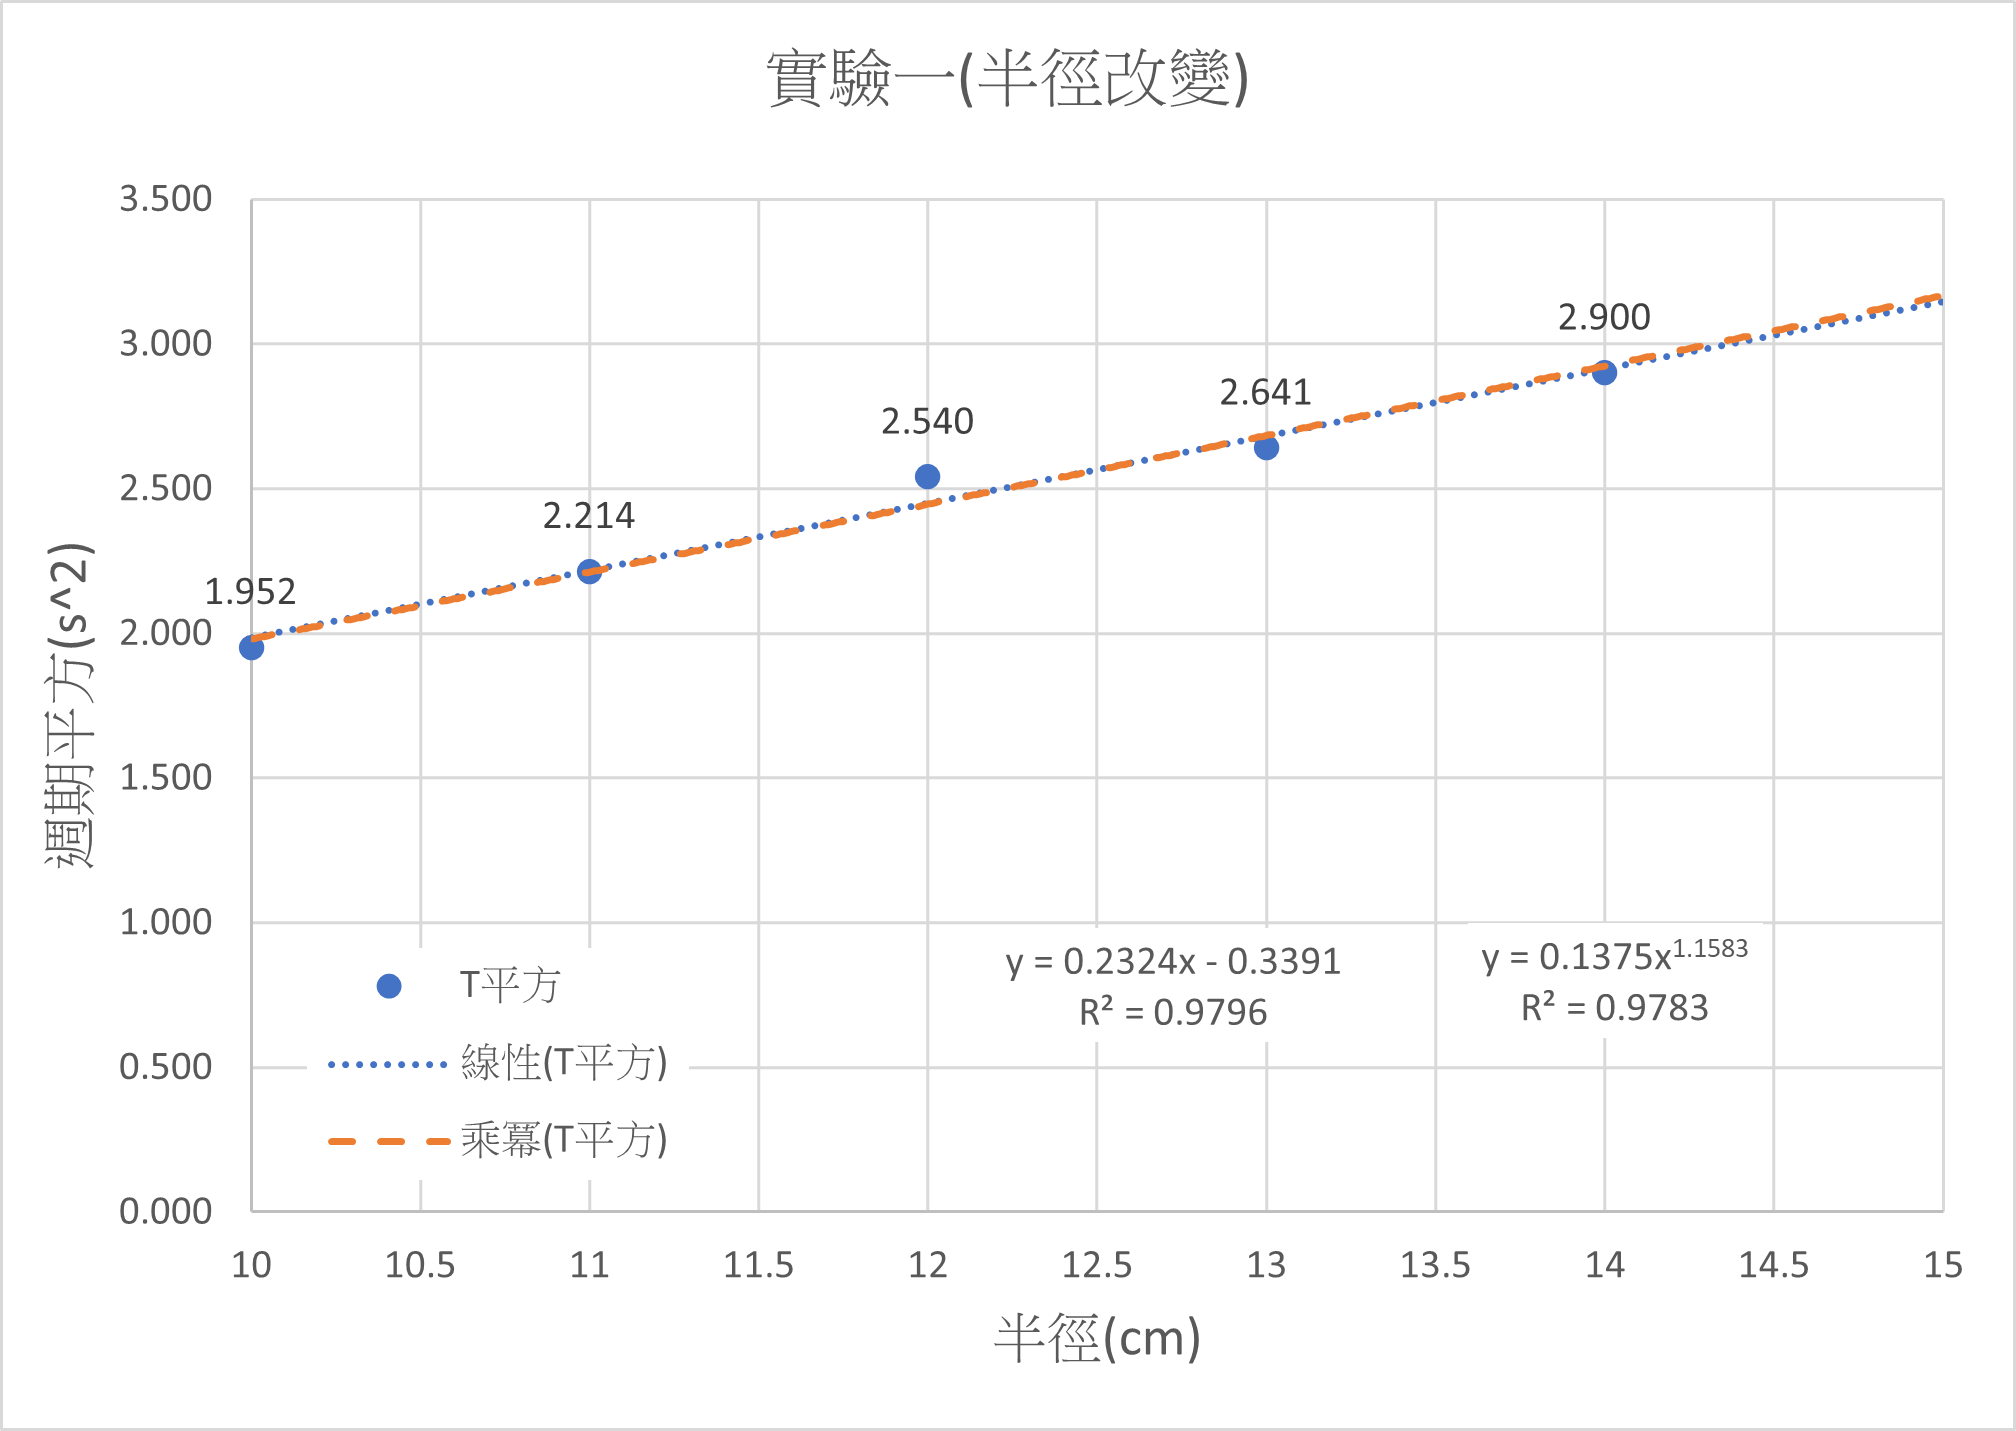
\includegraphics[width=0.8\linewidth]{向心力圖表/實驗一(半徑改變).png}
    \caption{半徑改變}
    \label{fig:半徑改變}
\end{figure}

%%%%%%%%%%%%%%%%%%%%%%%%%%%%%%實驗二%%%%%%%%%%%%%%%%%%%%%%%%%%%%%%%%%%%%%%%%%%%%%
\subsection{\textbf{實驗二}：固定旋轉半徑、旋轉砝碼質量，改變向心力}
旋轉砝碼質量:208.36g。旋轉半徑為:10cm
\begin{table}[h]
\centering
\begin{tabular}{cccc}
\hline
吊盤與砝碼質量m & 向心力F(dyne) & 週期T(s) & $\frac{1}{T^2}$ \\ \hline
19.99g   & 19590      & 2.579  & 0.130           \\
29.74g   & 29145      & 1.708  & 0.343           \\
39.54g   & 38749      & 1.429  & 0.489           \\
49.61g   & 48617      & 1.304  & 0.588           \\
59.35g   & 58163      & 1.242  & 0.648           \\ \hline
\end{tabular}
\end{table}

\begin{enumerate}
    \item 用\textit{excel}作圖後，可知趨勢線為$\frac{1}{T^2}=0.0032m^{1.3381}$(如\textit{Figure}\ref{fig:實驗二(改變向心力)與週期倒數作圖}所示)，而m的次方最接近的整數為$\beta=1$，此結果與理論預測相符合。
    \item 若改以$\frac{1}{T^2}=am+b$的表示方式，$a=0.0126$、$b=-0.055$，而$a$的理論值為$:\frac{980}{4\pi^2\times208.36\times10}=0.119$，所以本實驗誤差值為$5.8\%$

    \item 誤差來源與分析
    
    \begin{enumerate}
        \item 在本實驗，可以發現誤差相比與實驗一出現下降(9\%$\rightarrow$5.8\%)，一方面是因為改變了量測週期的器材，另一方面是因為相較於量測半徑，重量量測是使用電子秤，而能夠減小人為誤差。
        \item 若觀察Figure\ref{fig:實驗二(改變向心力)與週期倒數作圖} 數據的走向，能發現在砝碼重量增加時，週期平方倒數的數值漸漸下降，這跟理論預測有落差，我們認為可能的原因有二，分別為：彈簧的拉伸、砝碼與吊盤重量較小，角速度大，空氣阻力造成旋轉砝碼偏移，改變半徑。
    \end{enumerate}

    \item 盱衡所述，可以了解到在該實驗的誤差可能來自砝碼與吊盤的選擇上，之後可以選用重量較大的砝碼來當第一個數據點，使週期增加，降低速度，使空氣阻力下降，減少誤差。
\end{enumerate}

\begin{figure}[H]
    \centering
    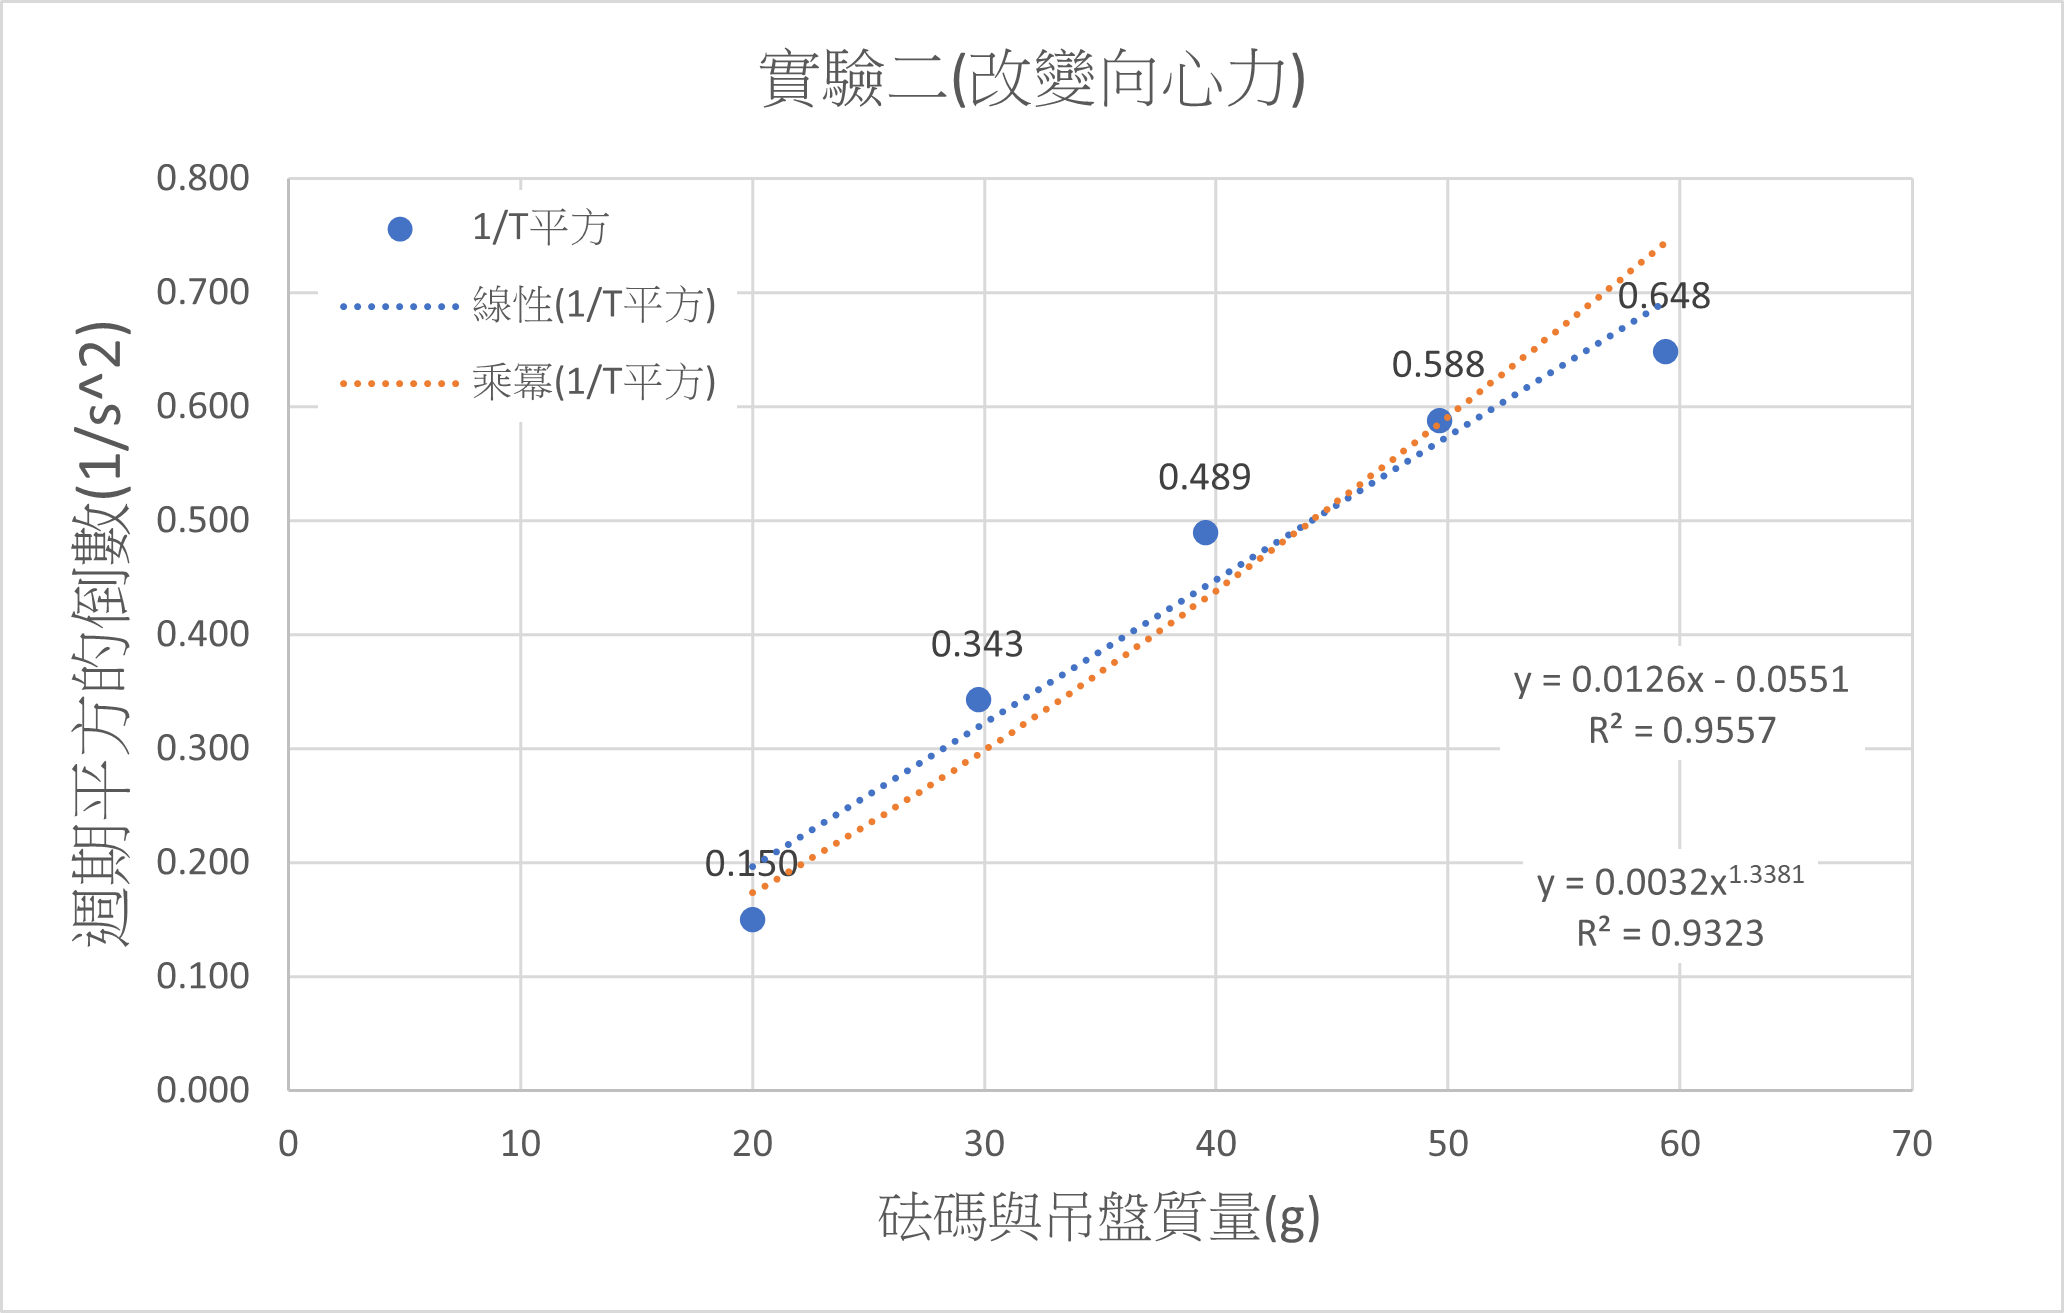
\includegraphics[width=0.8\linewidth]{向心力圖表/實驗二(改變向心力)與週期倒數作圖.png}
    \caption{實驗二(改變向心力)與週期倒數作圖}
    \label{fig:實驗二(改變向心力)與週期倒數作圖}
\end{figure}

\begin{figure}[H]
    \centering
    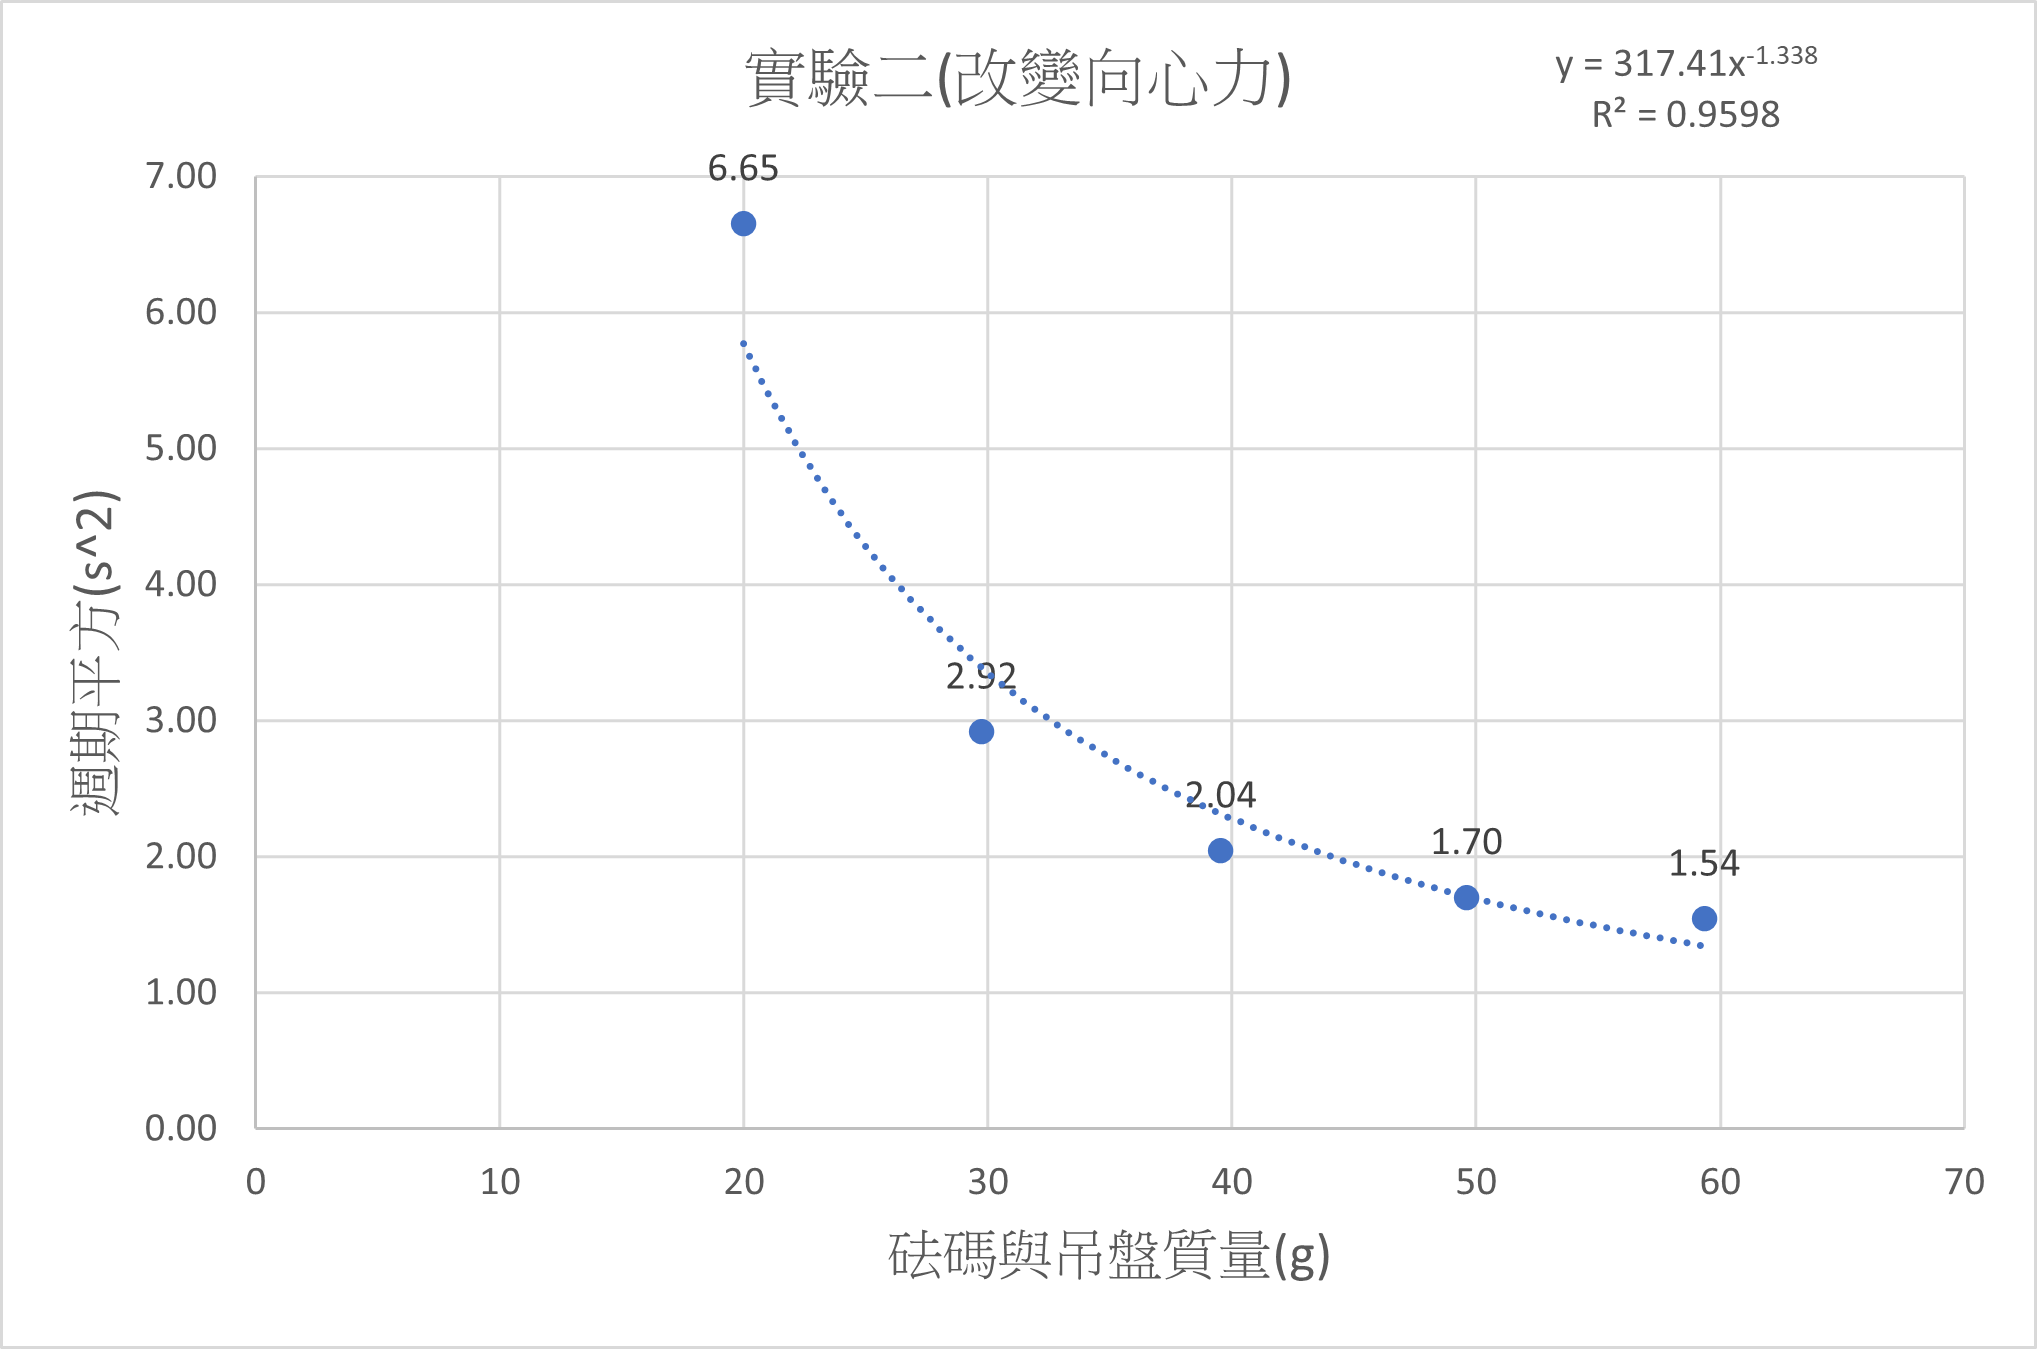
\includegraphics[width=0.8\linewidth]{向心力圖表/實驗二(改變向心力)與週期作圖.png}
    \caption{實驗二(改變向心力)與週期作圖}
    \label{fig:實驗二(改變心力)與週期作圖}
\end{figure}


%%%%%%%%%%%%%%%%%%%%%%%%%%實驗三%%%%%%%%%%%%%%%%%%%%%%%%%%%%%%%%%%%%
\subsection{\textbf{實驗三}:固定旋轉半徑、向心力，改變旋轉砝碼質量}
旋轉半徑為:10cm。吊盤與砝碼質量:39.79g$\Rightarrow{F=38994}$\textit{dyne}
\begin{table}[H]
\centering
\begin{tabular}{cccc}
\hline
旋轉砝碼質量M(g) & 向心力F(dyne) & 週期T(s) & $T^2$ \\ \hline
104.87g    & 38994      & 1.118  & 1.251 \\
156.69g    & 38994      & 1.212  & 1.469 \\
208.36g    & 38994      & 1.499  & 2.249 \\
255.09g    & 38994      & 1.558  & 2.427 \\
299.00g    & 38994      & 1.782  & 3.178 \\ \hline
\end{tabular}
\end{table}

\begin{enumerate}
    \item 用\textit{excel}作圖後，可知趨勢線為$T^2=0.0184M^{0.892}$(如\textit{Figure}\ref{fig:實驗三(改變砝碼質量)}所示)，而M的次方最接近的整數為$\beta=1$，此結果與理論預測相符合。
    \item 若改以$T^2=aM+b$的表示方式，$a=0.0099$、$b=0.0969$，而$a$的理論值為$:\frac{4\pi^2\times10}{39.79\times980}=0.0101$，所以本實驗誤差值為$0.2\%$
    \item 誤差來源分析:
    \begin{enumerate}
        \item 相比於實驗一、二，準確度更高，我們認為應該是在實驗過程中，半徑量測更為準確，吊盤與砝碼質量足夠重，使該實驗有良好的數據表現。
    \end{enumerate}
\end{enumerate}

\begin{figure}[H]
    \centering
    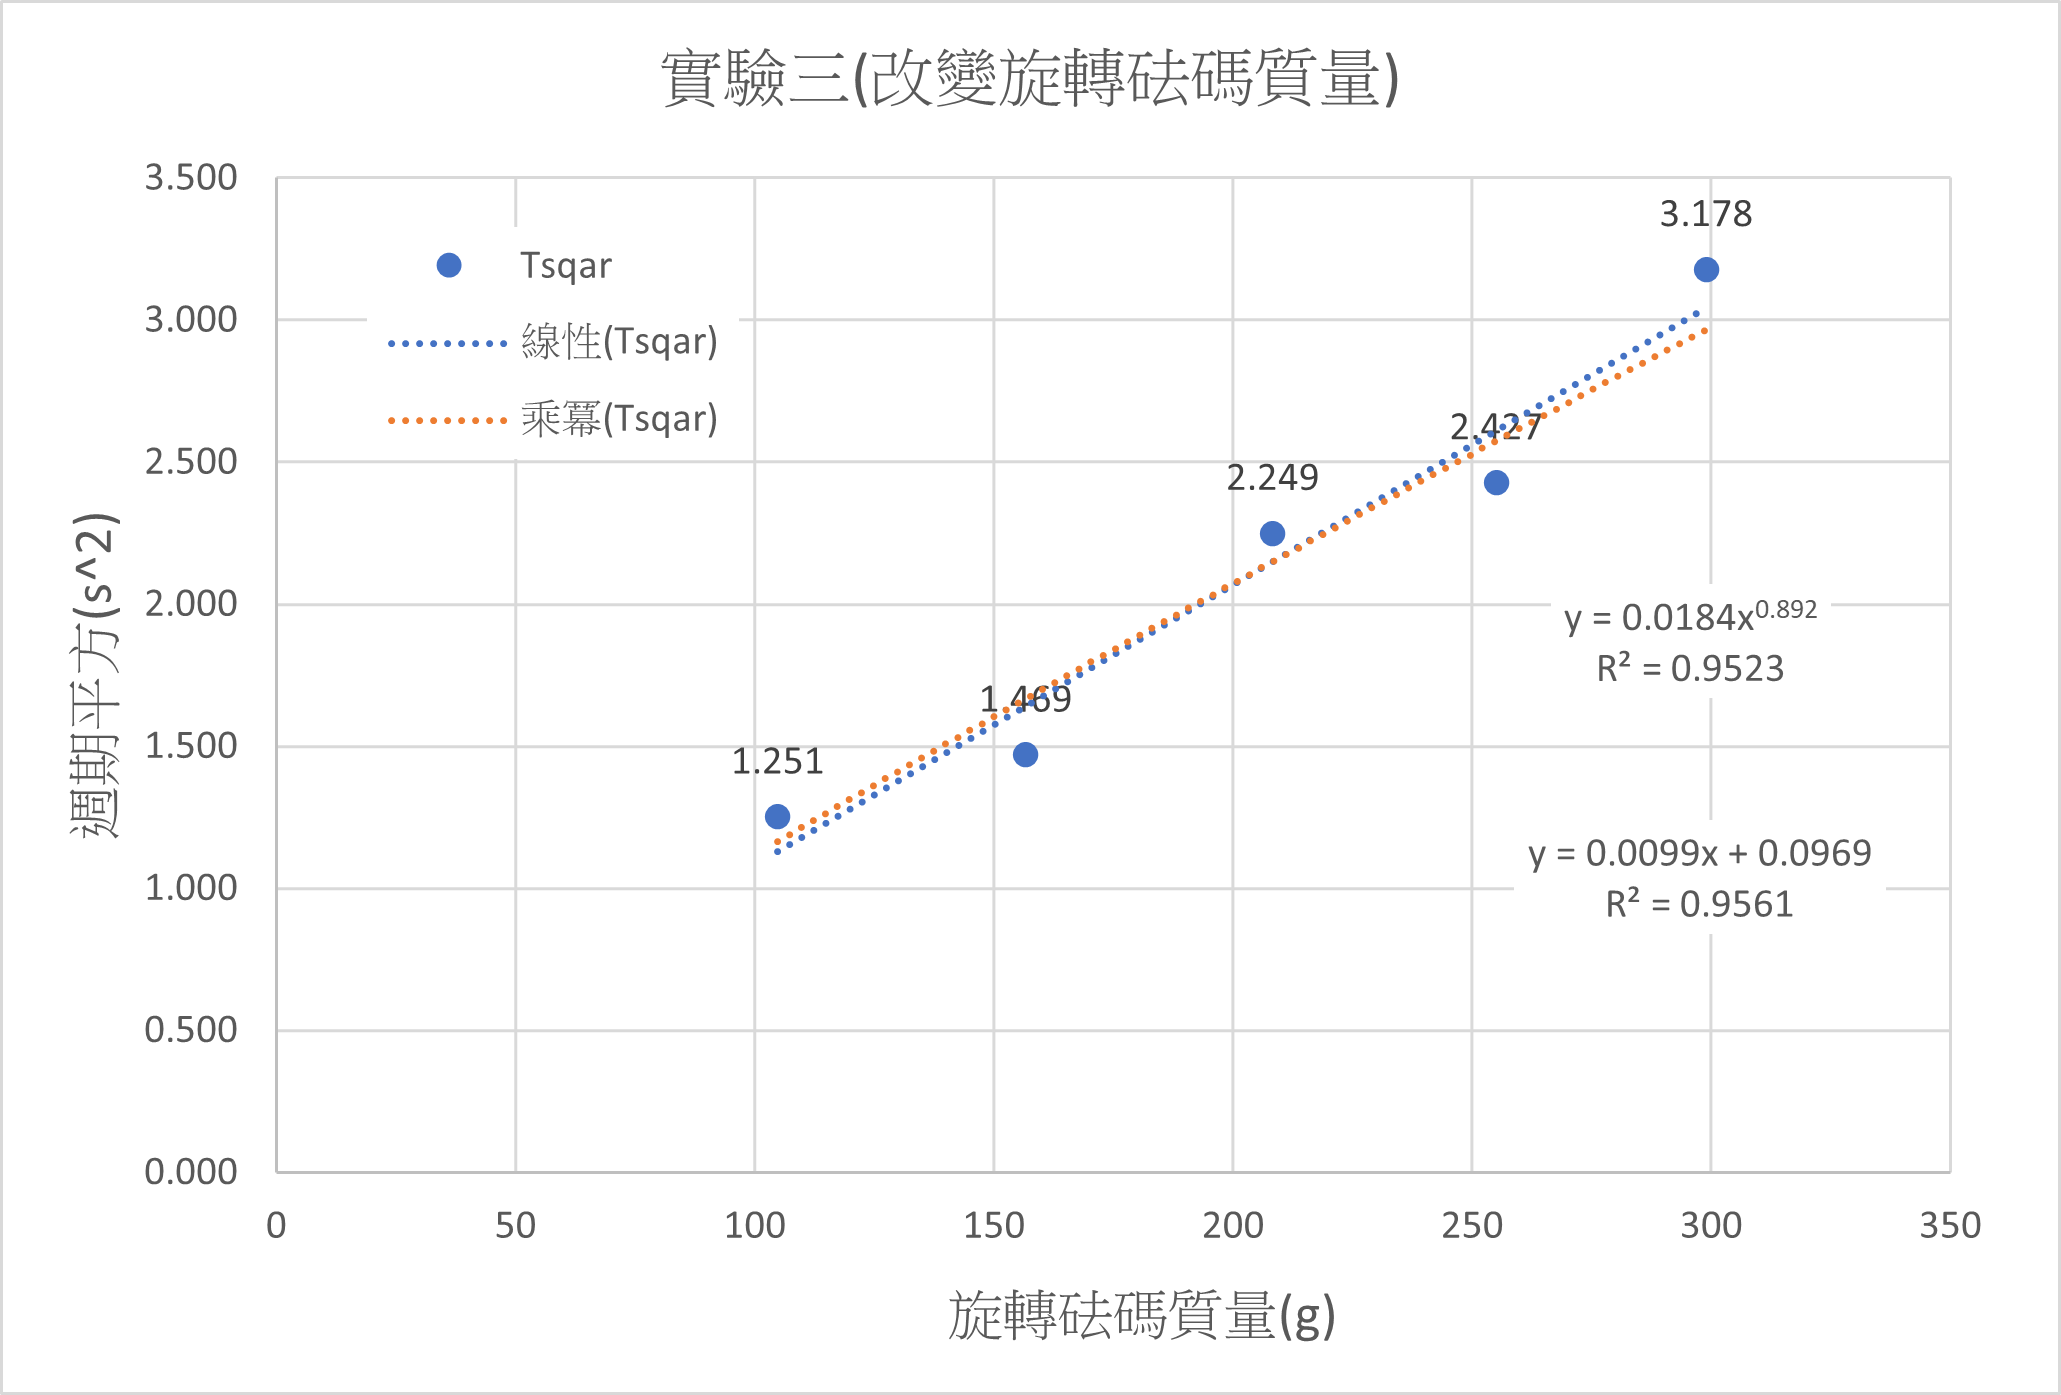
\includegraphics[width=0.8\linewidth]{向心力圖表/實驗三(改變砝碼質量).png}
    \caption{實驗三(改變砝碼質量)}
    \label{fig:實驗三(改變砝碼質量)}
\end{figure}

\newpage
%%%%%%%%%%%%%%%%%%%%%%%%%%%%%%%%%%%%%%%%%%%%%%%%%%%%%%%%%%%%%%%%

\section{\textbf{結果與討論}}
From \textit{Figure}~\ref{fig:半徑改變}, we can see that with every increase of $R$ (radius), the period squared $T^2$ also increases. This lines up well with the given formula. The graph clearly shows the connection between $T^2$ and $R$, which is proportional. We can also see that the change is quite linear, which means the acceleration is linearly increasing.

\textit{Figure}~\ref{fig:實驗二(改變心力)與週期作圖} shows a different scenario. The lines look parabolic. This means the acceleration is increasing as the total centripetal force increases (derived from the hanging mass's increase in value). The lines are not linear because $T^2$ is not proportional to $F$, as vaguely shown by our data. This means that when $F$ gets larger, the value of $T^2$ gets smaller. The non-linear increase in acceleration can also be explained by differentiating the function $T^2(F)$, which shows the acceleration is non-linear.

\textit{Figure}~\ref{fig:實驗二(改變向心力)與週期倒數作圖}, on the other hand, is the opposite. It is made by plotting $1/T^2$ instead of $T^2$. This flips the graph from non-linear to linear because the way the graph portrays changes has changed. In the second graph, we used $T^2$, which is disproportionate to $F$. In this graph, we use $1/T^2$, which aligns perfectly with the connection between $T^2$ and $F$, making the graph linear.

Since $T^2$ gets smaller as $F$ gets bigger, the value of $1/T^2$ gets larger. For example, $1/0.001 = 100$. This matches the graph, where $1/T^2$ increases as the force increases.

\textit{Figure}~\ref{fig:實驗三(改變砝碼質量)} is another linear graph. As the rotating weight’s mass increases, the period also increases. This aligns with the formula:
$T^2 = \frac{4 \pi^2 M R}{F}$
This shows that $T^2$ is proportional to the mass $M$ of the rotating weight. 

From the graphs, we can see that the values do not exactly match the expected line. The differences, ranging from 0.1 to 1 units, may be caused by instability in the rotating contraption's rotors, which can be wobbly and stuck at times. The discrepancy may also result from using a small number of data points for averaging. Increasing the number of experiments would make the output more reliable and precise.

誤差來源及改正:後來我們改用光電閘測週期,誤差便大幅減少。每轉一圈時,轉軸處會上下震動一次,無法順暢轉動,可能影響實驗週期測定。因此下次實驗前應檢查設備,避免不必要的誤差。過程中遇到物體旋轉前後位於不同位子,導致測量的旋轉半徑不準確,下次能等開始轉後記錄相對位置在測量。
%%%%%%%%%%%%%%%%%%%%%%%%%%%%%%%%%%%%%%%%%%%%%%%%%%%%%%%%%%%%%%%%%%%%%%%%%%%%%
\section*{\textbf{思考問題}}
\large
\noindent
$Q1:$綜合三種實驗，推斷F、M、$\omega$、r間的關係。\\
$A:$$F=Mr\omega^2$\\

\noindent
$Q2:$本實驗誤差來源，與影響。\\
$A:$本實驗誤差可能來自每次轉動時，質心與轉軸r 距離不完全相同，影響旋轉半徑的大小。每轉一圈時,轉軸處會上下震動一次,可能影響實驗週期測定Arduino的硬體問題,導致週期誤差大\\ 

\noindent
$Q3:$說明機車過彎時，要如何才不會飛出車道。\\
$A:$機車轉彎時要減速（增加旋轉時間、週期）、拉長距離（增加半徑）。\\

\noindent
$Q4:$日常生活中與向心力有關的應用。\\
$A:$洗衣機旋轉時，衣服緊貼在內壁（不碰到底部），正向力提供向心力及摩擦力。
%%%%%%%%%%%%%%%%%%%%%%%%%%%%%%%%%%%%%%%%%%%%%%%%%%%%%%%%%%%%%%%%%%%



\end{document}